\documentclass{beamer}
\usepackage[utf8]{inputenc}

\usetheme{Madrid}
\usecolortheme{default}
\usepackage{amsmath,amssymb,amsfonts,amsthm}
\usepackage{txfonts}
\usepackage{tkz-euclide}
\usepackage{listings}
\usepackage{adjustbox}
\usepackage{array}
\usepackage{tabularx}
\usepackage{gvv}
\usepackage{lmodern}
\usepackage{circuitikz}
\usepackage{tikz}
\usepackage{graphicx}
\usepackage{gensymb} % For using \degree symbol

\setbeamertemplate{page number in head/foot}[totalframenumber]

\title 
{2.3.6}
\date{September 12,2025}

\author 
{ADHARVAN KSHATHRIYA BOMMAGANI - EE25BTECH11003}

\begin{document}

\frame{\titlepage}

% Question Slide
\begin{frame}{Question}
Find the magnitude of each of the vectors $\vec{a}$ and $\vec{b}$, having the same magnitude such that the angle between them is $60\degree$ and their scalar product is $\frac{9}{2}$.
\end{frame}

% Step 1: Given Information
\begin{frame}{Theoretical Solution}
We are given:
\begin{itemize}
    \item Two vectors $\vec{a}$ and $\vec{b}$ with the same magnitude.
    \item The angle between them is $60\degree$.
    \item Their scalar product is:
    \begin{align}
        \vec{a}^T \vec{b} = \frac{9}{2}.
    \end{align}
\end{itemize}

Let the common magnitude be $r$, so
\begin{align}
    \|\vec{a}\| = \|\vec{b}\| = r.
\end{align}
\end{frame}

% Step 2: Cosine Formula
\begin{frame}{Theoretical Solution}
The formula for the dot product is:
\begin{align}
\cos\theta = \frac{\vec{a}^T \vec{b}}{\|\vec{a}\|\,\|\vec{b}\|}.
\end{align}

Since $\|\vec{a}\| = \|\vec{b}\| = r$, this simplifies to:
\begin{align}
\cos\theta = \frac{\vec{a}^T \vec{b}}{r^2}.
\end{align}

Given that $\theta = 60\degree$, we know $\cos 60\degree = \frac{1}{2}$.
Substituting values,
\begin{align}
\frac{1}{2} = \frac{\frac{9}{2}}{r^2}.
\end{align}
\end{frame}

% Step 3: Solve for r
\begin{frame}{Theoretical Solution}
Multiply throughout by $2r^2$:
\begin{align}
r^2 = 9.
\end{align}

Taking the positive square root (since magnitude cannot be negative),
\begin{align}
r = 3.
\end{align}

\[
\therefore \quad \|\vec{a}\| = \|\vec{b}\| = 3
\]

Thus, the magnitude of each vector is 3.
\end{frame}

\begin{frame}
    \vspace{5em}
\textbf{Two vectors with magnitude 3 and angle $\mathbf{60\degree}$ between them }
\begin{figure}[H]
    \centering
    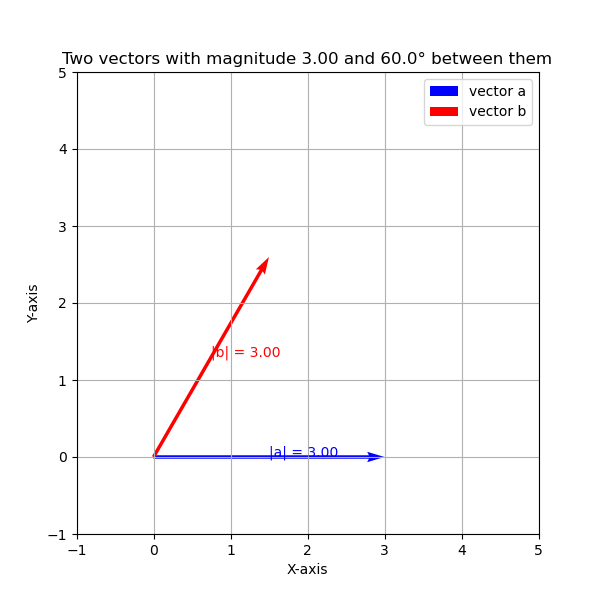
\includegraphics[width=0.4\columnwidth]{figs/fig1.png}
    \caption{Figure for 2.3.6}
    \label{fig1}
\end{figure}
\end{frame}

\end{document}
